% (c) 2012 Dimitrios Vrettos - d.vrettos@gmail.com
\section{Esercizi}
\subsection{Esercizi dei singoli paragrafi}
\subsubsection*{\thechapter.2 - Scrittura di un numero in una base qualsiasi}

\begin{esercizio}
\label{ese:4.1}
Stabilire il valore di verità delle seguenti proposizioni:
\begin{enumeratea}
\TabPositions{12cm}
\item la scrittura~1234 può esprimere un numero in base~4. \tab\boxV\quad\boxF
\item il valore numerico della cifra~2 nel numero~$(1523)_{6}$ espresso in base~10 è~72.\tab\boxV\quad\boxF
\item il valore numerico della cifra~3 nel numero~$(321)_{4}$ espresso in base~10 è~12. \tab\boxV\quad\boxF
\item il valore numerico di~$(321)_{4}$ espresso in base~10 è~57. \tab\boxV\quad\boxF
\end{enumeratea}
\end{esercizio}

\begin{esercizio}
\label{ese:4.2}
Scrivi il numero~$(3411)_{5}$ in forma polinomiale e trova il corrispondente numero decimale.
\[
(3411)_{5}=3\cdot 5^{\ldots }+\ldots \cdot 5^{2}+1\cdot5^{1}+\ldots\ldots =375+\ldots\ldots +5+\ldots%
\ldots\ldots\ldots =\ldots\ldots\]
\end{esercizio}

\begin{esercizio}[\Ast]
\label{ese:4.3}
Trasforma i seguenti numeri in un numero
decimale
\[(11101)_{2};\:\:(2001)_{3};\:\:(3023)_{4};\:\:(41)_{5};\:\:(3005)_{6}.\]
\end{esercizio}

\begin{esercizio}[\Ast]
\label{ese:4.4}
Trasforma i seguenti numeri scritti in base~2 in un numero decimale.
\[(110111)_{2};\:\:(1001)_{2};\:\:(111)_{2};\:\:(111111)_{2};\:\:(101)_{2}.\]
\end{esercizio}

\begin{esercizio}[\Ast]
\label{ese:4.5}
Trasforma i seguenti numeri scritti in base~16 in un numero decimale.
\[(20F)_{16};\:\:(AA)_{16};\:\:(19)_{16};\:\:(3E)_{16}.\]
\end{esercizio}

%%%%%%%%%%%%%%%%%%%%%%%%%%%%%%%%%%%%%%%%%%%%%

\begin{esercizio}
\label{ese:4.6}
Scrivere in base~2 i seguenti numeri in base dieci: 2; 4; 15; 12; 27; 33.

Risultati:
$(\ldots\ldots)_{2};\:\:(100)_{2};\:\:(\ldots\ldots)_{2};\:\:(1100)_{2};\:\:(\ldots\ldots\ldots)_{2};\:\:(100001)_{2}$.
\end{esercizio}

\begin{esercizio}
\label{ese:4.7}
Scrivere in base~3 i seguenti numeri: 2; 4; 15; 12; 27; 33.

Risultati:
$(2)_{3};\:\:(\ldots\ldots)_{3};\:\:(120)_{3};\:\:(\ldots\ldots)_{3};\:\:(1000)_{3};\:\:(\ldots\ldots\ldots)_{3}$.
\end{esercizio}

\begin{esercizio}
\label{ese:4.8}
Scrivere in base~4 i seguenti numeri: 2; 4; 15; 12; 27; 33.

Risultati:
$(\ldots\ldots)_{4};\:\:(10)_{4};\:\:(33)_{4};\:\:(\ldots\ldots)_{4};\:\:(\ldots\ldots)_{4};\:\:(201)_{4}$.
\end{esercizio}

\begin{esercizio}
\label{ese:4.9}
Scrivere in base~5 i seguenti numeri: 2; 4; 15; 12; 27; 33.

Risultati:
$(2)_{5};\:\:(\ldots\ldots)_{5};\:\:(\ldots\ldots)_{5};\:\:(22)_{5};\:\:(\ldots\ldots)_{5};\:\:(113)_{5}$.
\end{esercizio}

\begin{esercizio}
\label{ese:4.10}
Scrivere in base~6 i seguenti numeri: 2; 4; 15; 12; 27; 33.

Risultati:
$(\ldots\ldots)_{6};\:\:(4)_{6};\:\:(\ldots\ldots)_{6};\:\:(20)_{6};\:\:(\ldots\ldots)_{6};\:\:(\ldots\ldots)_{6}$.
\end{esercizio}

\begin{esercizio}
\label{ese:4.11}
Scrivere in base~7 i seguenti numeri decimali: 2; 4; 15; 12; 27; 33.

Risultati:
$(2)_{7};\;(\ldots\ldots)_{7};\;(\ldots\ldots)_{7};\;(\ldots\ldots)_{7};\;(\ldots\ldots)_{7};\;(45)_{7}$.
\end{esercizio}

\begin{esercizio}
\label{ese:4.12}
Scrivere in base~8 i seguenti numeri: 2; 4; 15; 12; 27; 33.

Risultati:
$(\ldots)_{8};\:\:(\ldots)_{2};\:\:(17)_{8};\:\:(\ldots\ldots)_{8};\:\:(33)_{8};\:\:(\ldots\ldots)_{8}$.
\end{esercizio}

\begin{esercizio}
\label{ese:4.13}
Scrivere in base~9 i seguenti numeri: 2; 4; 15; 12; 27; 33.

Risultati:
$(\ldots\ldots)_{9};\:\:(\ldots\ldots)_{9};\:\:(16)_{9};\:\:(\ldots\ldots)_{9};\:\:(\ldots\ldots)_{9};\:\:(36)_{9}$.

\end{esercizio}

\begin{esercizio}
\label{ese:4.14}
Scrivere in base~16 i seguenti numeri: 2; 4; 15; 12; 27; 33.

Risultati:
$(2)_{16};\:\:(\ldots\ldots)_{16};\:\:(F)_{16};\:\:(\ldots\ldots)_{16};\:\:(1B)_{16};\:\:(\ldots\ldots)_{16}$.
\end{esercizio}

\subsubsection*{4.3 - Conversione di un numero da una base diversa da~10 a un'altra base diversa da~10}

\begin{esercizio}
\label{ese:4.15}
Trasformare in base~7 i seguenti numeri scritti in base~4.
\[(103)_{4};\:\:(120)_{4};\:\:(203)_{4};\:\:(1301)_{4};\:\:(123)_{4};\:\:(301)_{4}.\]
Risultati:
$(25)_{7};\:\:(\ldots\ldots)_{7};\:\:(50)_{7};\:\:(\ldots\ldots)_{7};\:\:(36)_{7};\:\:(\ldots\ldots)_{7}$.
\end{esercizio}

\begin{esercizio}
\label{ese:4.16}
Trasformare in base~9 i seguenti numeri scritti in base~3.

\[(10002)_{3};\:\:(2020)_{3};\:\:(11201)_{3};\:\:(120122)_{3};\:\:(1001)_{3}.\]
Risultati:
$(102)_{9};\:\:(\ldots\ldots)_{9};\:\:(\ldots\ldots)_{9};\:\:(518)_{9};\:\:(\ldots\ldots)_{9}$.
\end{esercizio}

\begin{esercizio}
\label{ese:4.17}
Trasformare in base~16 i seguenti numeri scritti in base~4.

\[(133)_{4};\:\:(120)_{4};\:\:(203)_{4};\:\:(2301)_{4};\:\:(223)_{4}.\]
Risultati:
$(1F)_{16};\:\:(\ldots\ldots)_{16};\:\:(23)_{16};\:\:(\ldots\ldots)_{16};\:\:(2B)_{16}$.
\end{esercizio}

%%%%%%%%%%%%%%%%%%%%%%%%%%%%%%%%%%%%%%%%%%%%%%%%%%

\begin{esercizio}
\label{ese:4.18}
Convertire in base~4, 8 e~16 i seguenti numeri scritti in base~2:

\[(101)_{2};\quad(100011)_{2};\quad (1111110101)_{2};\quad (10100100)_{2};\quad (1101)_{2}.\]
\end{esercizio}


\begin{esercizio}
\label{ese:4.19}
Convertire in base~2 i seguenti numeri scritti in base~16:
\[(12)_{16};\quad (A)_{16};\quad (1C3)_{16};\quad (AB)_{16};\quad (223)_{16}.\]
\end{esercizio}


\begin{esercizio}[\Ast]
 \label{ese:4.20}
Perché un DVD scrivibile quando si compra dichiara una capacità di~$4,7\unit{GB}$ e
invece ha una capacità reale di~$4,3\unit{GiB}$? Un CD-R dichiara una
capacità di~$700\unit{MB}$. Qual è la sua capacità reale?
\end{esercizio}

\subsubsection*{4.4 - Operazioni in base diversa da dieci}

\begin{esercizio}
\label{ese:4.21}
Eseguire le seguenti addizioni in base~2.

 % (c) 2012 Dimitrios Vrettos - d.vrettos@gmail.com
\begin{tikzpicture}[ anchor=north west]

\begin{scope}[nodes={ text centered },cells={anchor=south}]
\matrix(a) [matrix of nodes]
{
1&1&1&1&0&1&$+$ \\
{}&1&0&1&1&0\\
};
\draw(a-2-1.south west)--(a-2-6.south east);

\begin{scope}[xshift=31.3mm]
\matrix(b) [matrix of nodes]
{
1&0&1&1&0&1&$+$ \\
{}&1&1&1&1&1\\
};
\draw(b-2-1.south west)--(b-2-6.south east);
\end{scope}

\begin{scope}[xshift=62.6mm]
\matrix(c) [matrix of nodes]
{
1&0&1&1&$+$ \\
{}&1&1&1&\\
};
\draw(c-2-1.south west)--(c-2-4.south east);
\end{scope}

\begin{scope}[xshift=86mm]
\matrix(d) [matrix of nodes]
{
1&0&1&1&$+$ \\
1&1&0&1&\\
1&0&1&1&\\
};
\draw(d-3-1.south west)--(d-3-4.south east);
\end{scope}

\begin{scope}[xshift=109.4mm]
\matrix(e) [matrix of nodes]
{
1&0&1&1&1&$+$ \\
1&1&0&0&1&\\
{}&1&1&0&0&\\
};
\draw(e-3-1.south west)--(e-3-5.south east);
\end{scope}
\end{scope}

\end{tikzpicture}

\end{esercizio}

\begin{esercizio}
\label{ese:4.22}
Eseguire le seguenti addizioni in base~5.

 % (c) 2012 Dimitrios Vrettos - d.vrettos@gmail.com

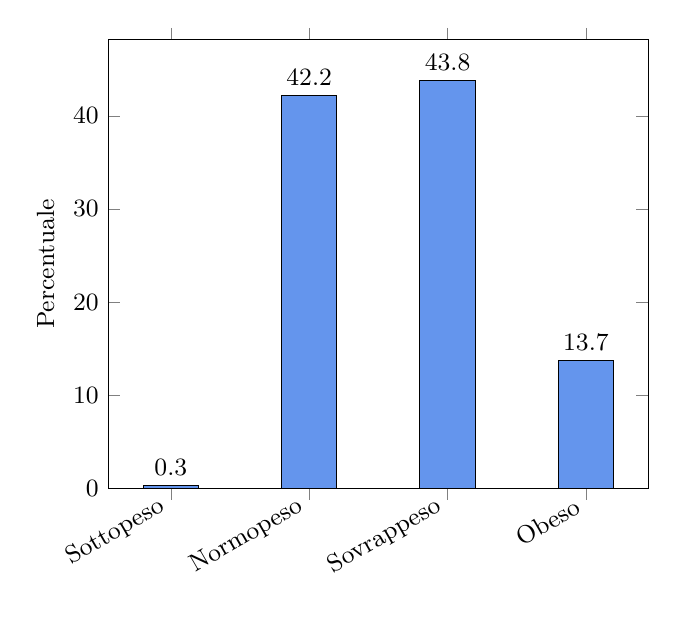
\begin{tikzpicture}[font=\small]
\begin{axis}[ymin=0,
ybar,
xtick=data,
ylabel=Percentuale,
x tick label style={rotate=30,anchor=east},
symbolic x coords={Sottopeso, Normopeso, Sovrappeso, Obeso},
bar width=20pt,enlarge x limits=0.15,nodes near coords,
nodes near coords align={vertical},
]
    \addplot[fill=CornflowerBlue,draw=black]
      coordinates{
	(Sottopeso, .3)
(Normopeso, 42.2)
(Sovrappeso, 43.8)
(Obeso,13.7)
      };
\end{axis}
\end{tikzpicture}

\end{esercizio}


\begin{esercizio}
\label{ese:4.23}
Eseguire le seguenti addizioni in base~3.

 % (c) 2012 Dimitrios Vrettos - d.vrettos@gmail.com
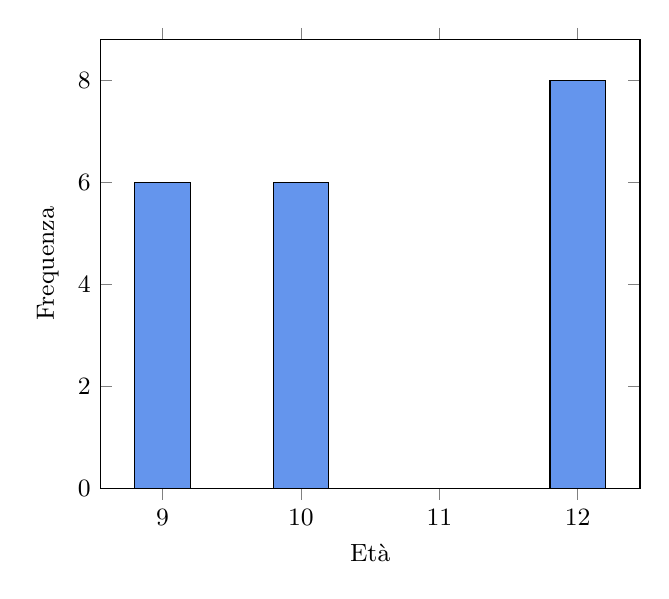
\begin{tikzpicture}[font=\small]

\begin{axis}[ymin=0,
ybar,
ylabel=Frequenza,
xlabel=Età,
bar width=20pt,
enlarge x limits=0.15,]

\addplot[fill=CornflowerBlue,draw=black]
      coordinates{
	(9, 6)
	(10,6)
	(12,8) };
\end{axis}
\end{tikzpicture}

\end{esercizio}

%%%%%%%%%%%%%%%%%%%%%%%%%%%%%%%%%%%%%%%%%%%%%
\begin{esercizio}
 \label{ese:4.24}
 Eseguire le seguenti sottrazioni in base~2.

 % (c) 2012 Dimitrios Vrettos - d.vrettos@gmail.com

\begin{tikzpicture}[x=10mm,y=10mm, font=\small,table nodes/.style={%
		rectangle,
		draw=black,
 		align=center,
   		minimum height=5mm,
     	text depth=0.5ex,
     	text height=1.5ex,
     	inner xsep=-1pt,
     	outer sep=0pt
	},
	table/.style={%
        matrix of nodes,
        row sep=-\pgflinewidth,
        column sep=-\pgflinewidth,
        nodes={%
            table nodes
        } }]

\matrix (first) [table,text width=7mm,name=table,row 2 column 2/.style=blue,row 5 column 4/.style=blue]
{
{}  & $-1$ & $+3$ & $-7$ & $+5$ & $-2$ & $+4$ & $+10$\\
$-1$ &[blue] 1 &{} &{} &{} &{} &{} &{} \\
$+3$ &{} &{} &{} &{} &{} &{} &{} \\
$-7$ &{} &{} &{} &{} &{} &{} &{} \\
$+5$ &{} &{} &{$0$} &{} &{} &{} &{} \\
$-2$ &{} &{} &{} &{} &{} &{} &{} \\
$+4$ &{} &{} &{} &{} &{} &{} &{} \\
$+10$ &{} &{} &{} &{} &{} &{} &{} \\
};

\end{tikzpicture}
\end{esercizio}

\begin{esercizio}
 \label{ese:4.25}
 Eseguire le seguenti sottrazioni in base~5.

 % (c) 2012 Dimitrios Vrettos - d.vrettos@gmail.com

\begin{tikzpicture}[x=10mm,y=10mm, font=\small, every state/.style={draw=CornflowerBlue}, every loop/.style={draw=Maroon}]
\draw (0,0) circle (2);
\node at (2,2) {$A$};
\node[state]  at (-1.5,0) {};
\node[state] (3) at (-.4,.8) {$+3$};
\node[state]  at (1.1,.5) {};
\node[state]  at (-.5,-.2) {};
\node[state] (10) at (1,-1) {$+10$};
\node[state] (7) at (-.5,-1.2) {$-7$};

\begin{scope}[->]
\path (3) edge[loop above] node{} ()
	(10) edge[loop above] node{} ()
   (7) edge[loop right] node {} ();

\end{scope}
\begin{scope}[-, Maroon]
\draw (10)--(3);
\end{scope}
\end{tikzpicture}
\end{esercizio}

\begin{esercizio}
 \label{ese:4.26}
 Eseguire le seguenti sottrazioni in base~3.

 % (c) 2012 Dimitrios Vrettos - d.vrettos@gmail.com
\begin{tikzpicture}[ anchor=north west]

\begin{scope}[nodes={ text centered },cells={anchor=south}]
\matrix(a) [matrix of nodes]
{
2&1&0&2&0&1&$-$ \\
{}&2&1&{2}&{1}&{2}\\
};
\draw(a-2-1.south west)--(a-2-6.south east);

\begin{scope}[xshift=31.3mm]
\matrix(b) [matrix of nodes]
{
2&0&2&1&0&1&$-$ \\
{}&{1}&{2}&{1}&{1}&{0}\\
};
\draw(b-2-1.south west)--(b-2-6.south east);
\end{scope}

\begin{scope}[xshift=62.6mm]
\matrix(c) [matrix of nodes]
{
2&2&1&1&$-$ \\
{}&2&0&2&\\
};
\draw(c-2-1.south west)--(c-2-4.south east);
\end{scope}

\begin{scope}[xshift=86mm]
\matrix(d) [matrix of nodes]
{
1&2&0&1&$-$ \\
{}&2&2&2&\\
};
\draw(d-2-1.south west)--(d-2-4.south east);
\end{scope}

\begin{scope}[xshift=109.3mm]
\matrix(e) [matrix of nodes]
{
2&1&0&0&1&$-$ \\
1&2&1&0&2&{}\\
};
\draw(e-2-1.south west)--(e-2-5.south east);
\end{scope}
\end{scope}

\end{tikzpicture}

\end{esercizio}

%%%%%%%%%%%%%%%%%%%%%%%%%%%%%%%%%%%%%%%%%%%%%%%

\begin{esercizio}
 \label{ese:4.27}
Moltiplicare in base~2:~\quad$111101_{2}\cdot~10110_{2}$;\quad
$101101_{2}\cdot~11111_{2}$;\quad~$1011_{2}\cdot~111_{2}$.
\end{esercizio}

\begin{esercizio}
 \label{ese:4.28}
Moltiplicare in base~5:~\quad$2401_{5}\cdot~42_{5}$;\quad
$431_{5}\cdot~34_{5}$;\quad~$214_{5}\cdot~41_{5}$.
\end{esercizio}

\begin{esercizio}
 \label{ese:4.29}
Moltiplicare in base~3:~\quad$10201_{3}\cdot~212_{3}$;\quad
$2101_{3}\cdot~212_{3}$;\quad~$1211_{3}\cdot~22_{3}$.
\end{esercizio}

\begin{esercizio}[\Ast]
\label{ese:4.30}
Eseguire le seguenti divisioni in base~2.
 \begin{multicols}{3}
 \begin{enumeratea}
  \item $11101_2:11_2$;
  \item $1011101_2:100_2$;
  \item $100011_2:10_2$.
 \end{enumeratea}
 \end{multicols}
\end{esercizio}

\begin{esercizio}[\Ast]
\label{ese:4.31}
Eseguire le seguenti divisioni in base~5.
 \begin{multicols}{3}
 \begin{enumeratea}
  \item $2304_5:43_5$;
  \item $3310_5:24_5$;
  \item $2012_5:31_5$.
 \end{enumeratea}
 \end{multicols}
\end{esercizio}

\subsection{Risposte}

\paragraph{\thechapter.3.} 29; 55; 203; 21; 653.

\paragraph{\thechapter.4.} 55; 9; 7; 63; 5.

\paragraph{\thechapter.5.} 527; 170; 25; 62.

\paragraph{\thechapter.20.} $667,57\unit{MiB}$.

\paragraph{\thechapter.30.}
a)~$\text{Q}=11_2$,~~$\text{R}=1_2$;\quad b)~$\text{Q}=1011_2$,~~$\text{R}=1_2$;\quad c)~$\text{Q}=10001_2$,~~$\text{R}=0_2$.

\paragraph{\thechapter.31.}
a)~$\text{Q}=24_5$,~~$\text{R}=12_5$;\quad b)~$\text{Q}=112_5$,~~$\text{R}=12_5$;\quad c)~$\text{Q}=31_5$,~~$\text{R}=1_5$.
